\chapter{Local Flatness, Geodesics, Rindler Space, and Schwarzschild}

This lecture begins in the middle of an earlier discussion, and it is best to keep that tone. We do not begin with black holes. We begin by sorting out what flattening can mean, what topology can obstruct, and what freedom remains in the choice of metric. From there the lecture narrows to geodesic coordinates, where curvature becomes a statement about second derivatives of the metric; then it turns that geometry into particle dynamics through the action; and only after that does it introduce Rindler space as the simplest horizon-bearing geometry, in order to prepare the Schwarzschild metric. These notes follow Leonard Susskind's lecture, with the present edition curated with help from LazyingArt LLC and Video2Book.

\section{Topology, Flattening, and What the Metric Can Change}

We begin with a carry-over point from the previous lecture. In two dimensions the Gaussian curvature has only one independent component, so one may speak simply of the curvature scalar \(K\). On the standard torus, the outer rim has positive curvature, the inner region has negative curvature, and the two balance so that the integral over the whole surface vanishes. The lecture uses this to separate a global topological statement from any particular local shape one may draw in three-dimensional space.

In the lecture's normalization, the sample values are
\begin{align}
\int K\,dA &= +1 && \text{sphere}, \\
\int K\,dA &= 0 && \text{torus}, \\
\int K\,dA &= -1 && \text{torus with two holes}, \\
\int K\,dA &= -2 && \text{torus with three holes}.
\end{align}
The point is not to prove Gauss--Bonnet carefully here. The point is that the integrated curvature depends only on the topology. One may put bulges into a torus, stretch it into a coffee cup, or otherwise distort it, but one does not change this integral.

That immediately suggests the right question. If the plane has zero curvature everywhere, and therefore zero integrated curvature, then among these examples only the torus has any chance of being flattened. But zero integrated curvature does not by itself prove that a given torus, with its given metric, can be unfolded into a plane. It only says that topology does not forbid it. The lecture then makes the stronger statement: one can put a different metric on the torus, a metric that is flat everywhere.

The next example is more delicate and more instructive. Take a sphere and remove one point. Can that be made flat? The answer is yes, provided we do not insist on the standard round metric of the sphere. The sphere minus one point can be mapped one-to-one onto the plane, and then it can inherit the flat metric of the plane. The price is that the inherited metric is singular at the removed point.

\begin{figure}[t]
\centering
\begin{tikzpicture}[scale=0.95]
\draw (-3.2,-2) -- (6.0,-2);
\draw (0,0) circle (2);
\fill (0,2) circle (0.05);
\fill (0,-2) circle (0.05);
\fill (1.9,0.62) circle (0.05);
\fill (5.2,-2) circle (0.05);
\draw (0,2) -- (5.2,-2);
\node[above] at (0,2) {$N$};
\node[below] at (0,-2) {$S$};
\node[right] at (1.9,0.62) {$P$};
\node[below] at (5.2,-2) {$P'$};
\node[below left] at (-2.8,-2) {plane};
\node at (0,0) {sphere};
\end{tikzpicture}
\caption{A sphere tangent to a plane, with the north-pole projection used to identify the sphere minus one point with the plane.}
\end{figure}

The construction is the usual one. Place the sphere tangent to a plane. For any point \(P\) on the sphere, draw the straight line from the north pole through \(P\), and continue it until it reaches the plane. In this way every point of the sphere except the north pole is sent to a unique point of the plane. If we start with the standard flat metric on the plane,
\begin{equation}
ds^2 = dx^2 + dy^2,
\end{equation}
we may pull that metric back to the sphere minus the north pole.

The resulting geometry is flat, but singular. A point very near the north pole maps very far out on the plane. Therefore neighboring points near the north pole acquire very large distances in the pulled-back metric, and the metric components diverge there. This is exactly what the lecture wants us to see: flattening the sphere minus one point is possible, but only at the price of a singular metric at the missing point.

A student then pushes on a different issue. Could one scramble points so violently that one maps a square to a line, or two-dimensional space to one-dimensional space, by interleaving decimal expansions? Set-theoretically one can write such monstrous correspondences. But they are not continuous, not differentiable, and they destroy the local notion of neighboring points. Susskind's verdict is the right one: this is not a proper coordinate transformation. Once we exclude such pathological maps, we are naturally led to the right local notion of flattening.

\section{Geodesic Coordinates and Where Curvature Lives}

The right local answer is geodesic coordinates. Pick a point \(p\) in curved space. Through that point draw two perpendicular geodesics and use them as local axes. For a nearby point, drop perpendicular geodesics to those axes and use the geodesic distances as coordinates. This is only a local construction, but it is the local construction that most closely imitates Cartesian coordinates in flat space.

\begin{figure}[t]
\centering

\includegraphics[width=0.74\textwidth]{lecture_11_figure_02.png}
\caption{Blackboard sketch of the local geodesic-coordinate construction at a point.}
\end{figure}

\begin{figure}[t]
\centering
\begin{tikzpicture}[scale=1.0]
\draw (-3.2,0.35) .. controls (-1.8,0.75) and (-0.4,0.55) .. (0.15,0.42)
                     .. controls (1.0,0.22) and (2.0,0.12) .. (3.3,0.45);
\draw (-0.45,-2.6) .. controls (-0.75,-1.2) and (-0.20,-0.2) .. (0.15,0.42)
                    .. controls (0.55,1.0) and (0.85,1.9) .. (1.00,2.75);
\fill (0.15,0.42) circle (0.06);
\draw (0.03,0.42) -- (0.15,0.56) -- (0.27,0.42) -- (0.15,0.28) -- cycle;
\fill (1.55,1.15) circle (0.05);
\draw[dashed] (1.55,1.15) -- (1.08,0.60);
\draw[dashed] (1.55,1.15) -- (0.65,1.55);
\node[below] at (0.15,0.22) {$p$};
\node[right] at (1.62,1.15) {$q$};
\node[below] at (1.15,0.52) {$x$};
\node[left] at (0.75,1.45) {$y$};
\node[below right] at (2.7,0.28) {geodesic axis};
\node[right] at (0.95,2.4) {geodesic axis};
\end{tikzpicture}
\caption{A clean redraw of the local picture: two perpendicular geodesics through \(p\), with nearby coordinates assigned by geodesic distances.}
\end{figure}

The key local facts are
\begin{equation}
g_{ij}(p)=\delta_{ij},
\qquad
\partial_k g_{ij}(p)=0.
\end{equation}
Since the Christoffel symbols are built from first derivatives of the metric, it follows immediately that
\begin{equation}
\Gamma^{i}{}_{jk}(p)=0.
\end{equation}
This is local flatness in the precise sense relevant for the lecture: at a chosen point the metric looks Euclidean, and its first derivatives vanish.

\subsection{Question \& Answer}

Question: if the Christoffel symbols vanish at the point, why does the curvature not vanish there as well?

Answer: because the Riemann tensor has two kinds of terms. Schematically,
\begin{equation}
R \sim \partial \Gamma + \Gamma\Gamma.
\end{equation}
The blackboard summary is worth keeping, because it captures the logic of the lecture rather than a fully indexed formula.

\begin{figure}[t]
\centering

\includegraphics[width=0.62\textwidth]{lecture_11_figure_03.png}
\caption{Blackboard summary: curvature is schematically built from \(\partial\Gamma\) and \(\Gamma\Gamma\), hence from second and first derivatives of the metric.}
\end{figure}

Since \(\Gamma^{i}{}_{jk}(p)=0\), the quadratic \(\Gamma\Gamma\) terms vanish at \(p\). But the derivative term does not vanish in general, because it contains derivatives of the Christoffel symbols, and therefore second derivatives of the metric. In the same schematic spirit,
\begin{equation}
R \sim \partial^2 g + (\partial g)^2.
\end{equation}
At the chosen point in geodesic coordinates the second term drops out, and what survives is the dependence on second derivatives:
\begin{equation}
R(p)\sim \partial^2 g(p).
\end{equation}

This is the real lesson. Curvature is not first-derivative data. By a suitable choice of coordinates we can kill the first derivatives of the metric at one point, and with them the Christoffel symbols. What we cannot kill in general are the second derivatives. That is where the intrinsic curvature lives.

\section{Geodesics, Local Extremality, and the Particle Action}

The discussion now shifts, very naturally, from local curvature to motion. A geodesic is not safely defined as the globally shortest path between two points. The official rule is more robust:
\begin{equation}
u^\nu \nabla_\nu u^\mu = 0,
\end{equation}
where \(u^\mu = dx^\mu/d\tau\) is the tangent vector to the curve. The tangent vector is covariantly constant along the curve. That statement survives even when the naive shortest-path slogan becomes misleading.

\subsection{Question \& Answer}

Question: is a geodesic necessarily a minimum of length, or of proper time?

Answer: only locally, and not always as a minimum. The lecture's example is a symmetric hill in ordinary two-dimensional space. Between two symmetrically placed points there are typically two stable geodesics, one going around one side and one around the other, and there is also a third geodesic running straight over the summit. The summit path is a geodesic in the official sense, but it is an unstable local maximum of length, not a minimum.

\begin{figure}[t]
\centering
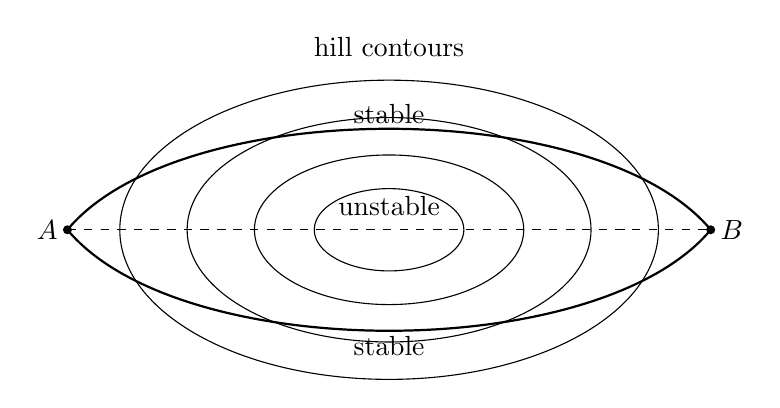
\begin{tikzpicture}[scale=0.95]
\draw (0,0) ellipse (1.0 and 0.55);
\draw (0,0) ellipse (1.8 and 1.0);
\draw (0,0) ellipse (2.7 and 1.5);
\draw (0,0) ellipse (3.6 and 2.0);
\fill (-4.3,0) circle (0.06);
\fill (4.3,0) circle (0.06);
\node[left] at (-4.3,0) {$A$};
\node[right] at (4.3,0) {$B$};
\draw[thick] (-4.3,0) .. controls (-2.8,1.8) and (2.8,1.8) .. (4.3,0);
\draw[thick] (-4.3,0) .. controls (-2.8,-1.8) and (2.8,-1.8) .. (4.3,0);
\draw[dashed] (-4.3,0) .. controls (-1.6,0.0) and (1.6,0.0) .. (4.3,0);
\node at (0,2.45) {hill contours};
\node at (0,0.32) {unstable};
\node at (0,1.55) {stable};
\node at (0,-1.55) {stable};
\end{tikzpicture}
\caption{The hill example from the lecture: two stable side geodesics and one unstable summit geodesic.}
\end{figure}

That example does the needed work. It breaks the automatic identification of geodesic with absolute minimum, and prepares the move to the action principle.

The action for a point particle is defined by
\begin{equation}
S = -m \int d\tau,
\end{equation}
with
\begin{equation}
d\tau^2 = g_{\mu\nu}(x)\,dx^\mu dx^\nu.
\end{equation}
This is not something to be derived from a previous principle in the lecture; it is taken as the definition of the relativistic action for a free particle in a metric background.

Now choose one coordinate, \(x^0=t\), and rewrite the action in terms of coordinate time. First decompose the quadratic form:
\begin{equation}
g_{\mu\nu}\,dx^\mu dx^\nu
=
g_{00}\,dt^2 + 2g_{0i}\,dt\,dx^i + g_{ij}\,dx^i dx^j.
\end{equation}
Then divide by \(dt^2\) inside the square root and write \(\dot x^i = dx^i/dt\). The action becomes
\begin{align}
S
&=
-m\int \sqrt{g_{\mu\nu}(x)\,dx^\mu dx^\nu}
\\
&=
-m\int dt\,
\sqrt{g_{00}+2g_{0i}\dot x^i+g_{ij}\dot x^i\dot x^j}.
\end{align}
So the coordinate-time Lagrangian is
\begin{equation}
L(x,\dot x)
=
-m\sqrt{g_{00}+2g_{0i}\dot x^i+g_{ij}\dot x^i\dot x^j}.
\end{equation}

This is more cumbersome than the nonrelativistic Lagrangian because everything sits inside a square root. But conceptually it is ordinary mechanics again: \(L\) depends on coordinates through the metric, and on velocities through the quadratic form. One may write the Euler--Lagrange equations, and after the somewhat annoying conversion between \(t\)-derivatives and \(\tau\)-derivatives, one recovers the geodesic equation in its standard form,
\begin{equation}
\frac{d^2x^\mu}{d\tau^2}
+
\Gamma^\mu_{\nu\rho}\,
\frac{dx^\nu}{d\tau}
\frac{dx^\rho}{d\tau}
=0.
\end{equation}
The lecture does not carry this conversion to the end on the board, and that is fine. The main point is the equivalence of logic: stationary proper time and stationary action are the same principle for a free particle in any metric.

\section{Weak Fields and the Meaning of \texorpdfstring{$g_{00}$}{g00}}

Having obtained the general Lagrangian, the lecture immediately simplifies it to the weak-field, low-velocity regime. This is the bridge back to Newtonian physics.

Assume that only the time-time component of the metric differs appreciably from its flat value, and write
\begin{equation}
g_{00}=1+\delta g_{00},
\qquad
g_{0i}=0,
\qquad
g_{ij}\approx -\delta_{ij}.
\end{equation}
Then the square root becomes a square root of \(1\) plus something small:
\begin{equation}
L \approx -m\sqrt{1+\delta g_{00}-\dot x^{\,2}}.
\end{equation}
Using \(\sqrt{1+s}\approx 1+s/2\) for small \(s\), we obtain
\begin{align}
L
&\approx
-m\left(1+\frac{\delta g_{00}}{2}-\frac{\dot x^{\,2}}{2}\right)
\\
&\approx
-m-\frac{m\,\delta g_{00}}{2}+\frac{m\dot x^{\,2}}{2}.
\end{align}

\begin{figure}[t]
\centering

\includegraphics[width=0.70\textwidth]{lecture_11_figure_05.png}
\caption{Weak-field expansion of the point-particle Lagrangian as it appears on the board.}
\end{figure}

The blackboard line is slightly loose on the second step: the middle term appears without an explicit factor of \(m\). But the first line is clear, and the intended decomposition is equally clear. We have a constant term, a term depending only on the metric perturbation, and the familiar kinetic term \(\frac12 m\dot x^{\,2}\).

Now the Newtonian interpretation comes back. The Lagrangian is \(L=T-V\), so the terms that do not depend on velocity correspond to minus the potential energy. Therefore the perturbation in \(g_{00}\) plays the role of the gravitational potential, up to the usual additive constant and the sign bookkeeping that Susskind explicitly treats a little loosely:
\begin{equation}
g_{00}\approx \text{const}+2\Phi,
\qquad
\Phi \approx \frac{\delta g_{00}}{2}.
\end{equation}
The reason for writing \(\delta g_{00}\) rather than simply \(g_{00}\) is that only derivatives matter physically in the Newtonian comparison. One may always add a constant to the potential, and correspondingly to \(g_{00}\), without changing the force.

For a point mass in Newtonian gravity,
\begin{equation}
\Phi(r)=-\frac{GM}{r}.
\end{equation}
This is exactly the relation that will later motivate the time-time coefficient of the Schwarzschild metric.

\section{Uniform Acceleration and Rindler Space}

At this point the lecture finally announces black holes, and then immediately postpones them. Before we discuss the Schwarzschild metric, we are told, we must understand accelerated frames in relativity, because horizons already appear there.

In Newtonian mechanics one imagines a uniformly accelerated observer following a parabola,
\[
x=x_0+v_0 t+\frac12 a t^2.
\]
But this cannot be right in special relativity. If \(a\) were constant in that naive sense, the velocity would eventually exceed the speed of light. The relativistically correct uniformly accelerated worldline is instead a hyperbola:
\begin{equation}
x^2-t^2=R^2.
\end{equation}
The crucial virtue of this curve is that it is Lorentz-invariant. A Lorentz transformation moves a point on the hyperbola to another point on the same hyperbola, so the observer feels the same proper acceleration all along the path.

\begin{figure}[t]
\centering
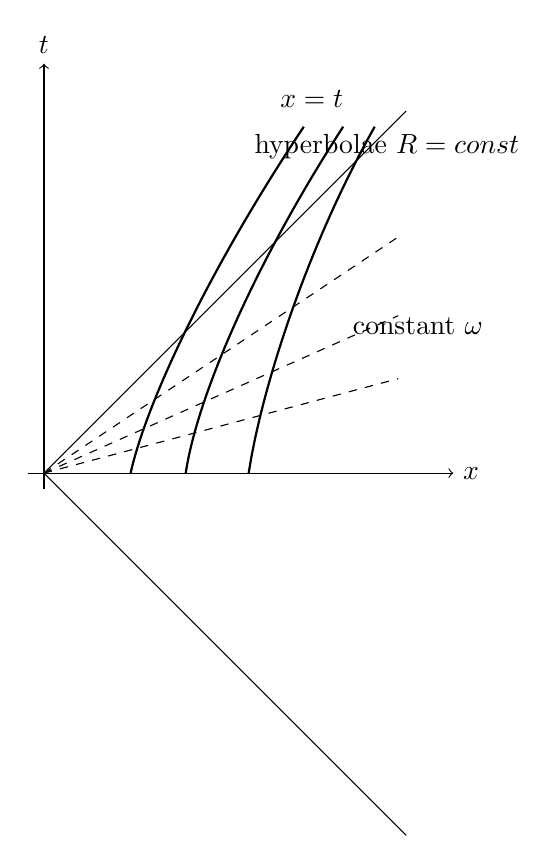
\begin{tikzpicture}[scale=1.0]
\draw[->] (-0.2,0) -- (5.2,0) node[right] {$x$};
\draw[->] (0,-0.2) -- (0,5.2) node[above] {$t$};
\draw[thin] (0,0) -- (4.6,4.6);
\draw[thin] (0,0) -- (4.6,-4.6);
\draw[thick] (1.1,0.0) .. controls (1.3,0.9) and (2.1,2.6) .. (3.3,4.4);
\draw[thick] (1.8,0.0) .. controls (1.95,1.0) and (2.7,2.7) .. (3.8,4.4);
\draw[thick] (2.6,0.0) .. controls (2.75,1.0) and (3.3,2.8) .. (4.2,4.4);
\draw[dashed] (0,0) -- (4.5,1.2);
\draw[dashed] (0,0) -- (4.5,2.0);
\draw[dashed] (0,0) -- (4.5,3.0);
\node at (3.4,4.75) {$x=t$};
\node[below right] at (3.8,2.1) {constant \(\omega\)};
\node[right] at (2.55,4.15) {hyperbolae \(R=\text{const}\)};
\end{tikzpicture}
\caption{The right Rindler wedge of Minkowski space: light cone, hyperbolic worldlines \(R=\text{const}\), and rays of constant Rindler time \(\omega\).}
\end{figure}

A whole accelerated reference frame is built by taking a family of such hyperbolae. The important point is that different members of the family do not have the same proper acceleration. The deeper in one goes toward the origin of the Minkowski diagram, the larger the proper acceleration becomes. In the lecture the scaling is described schematically as \(a\sim 1/R\). So this is the best relativistic analogue of a uniformly accelerated frame: acceleration is constant along each worldline, but not the same from one worldline to another.

Now introduce the Rindler coordinates by analogy with polar coordinates. In Euclidean geometry we write \(x=R\cos\theta\), \(y=R\sin\theta\). For the hyperbolic problem we replace circular functions with hyperbolic ones:
\begin{equation}
x=R\cosh\omega,
\qquad
t=R\sinh\omega.
\end{equation}
Here \(R\) labels which hyperbola we are on, and \(\omega\) plays the role of time for the accelerated observer. Unlike an ordinary angle, \(\omega\) ranges from \(-\infty\) to \(+\infty\).

Differentiating gives
\begin{align}
dx &= \cosh\omega\,dR + R\sinh\omega\,d\omega, \\
dt &= \sinh\omega\,dR + R\cosh\omega\,d\omega.
\end{align}
Now substitute into the Minkowski line element in \(1+1\) dimensions:
\begin{equation}
d\tau^2=dt^2-dx^2.
\end{equation}
The cross terms cancel, and using \(\cosh^2\omega-\sinh^2\omega=1\) we find
\begin{align}
d\tau^2
&=
(\sinh^2\omega-\cosh^2\omega)\,dR^2
+
R^2(\cosh^2\omega-\sinh^2\omega)\,d\omega^2
\\
&=
R^2\,d\omega^2-dR^2.
\end{align}
The transverse coordinates \(y\) and \(z\) are unaffected by the boost, so the full line element is
\begin{equation}
d\tau^2 = R^2\,d\omega^2 - dR^2 - dy^2 - dz^2.
\end{equation}

This is still flat spacetime. Nothing gravitating has been introduced. But in these coordinates \(g_{\omega\omega}=R^2\), so from the accelerated point of view there is an effective gravitational field pulling freely moving bodies toward \(R=0\). The right wedge \(R>0\) is what the lecture calls Rindler space.

\subsection{Question \& Answer}

Question: what does the outside observer see when a rock is dropped, and what does the rock see?

Answer: the rock moves inertially, along a straight line in Minkowski space. The accelerated observers are the ones being forced off inertial motion. So from their point of view the rock falls toward the horizon at \(R=0\). But \(R=0\) is not an ordinary place in Rindler time. It is reached only at infinite \(\omega\).

\begin{figure}[t]
\centering
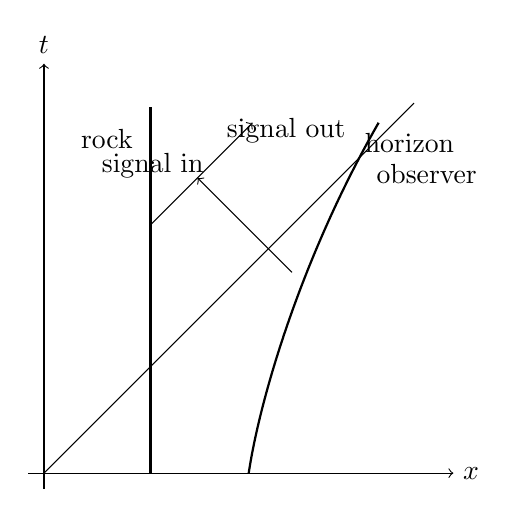
\begin{tikzpicture}[scale=1.0]
\draw[->] (-0.2,0) -- (5.2,0) node[right] {$x$};
\draw[->] (0,-0.2) -- (0,5.2) node[above] {$t$};
\draw[thin] (0,0) -- (4.7,4.7);
\draw[thick] (2.6,0.0) .. controls (2.75,1.0) and (3.3,2.8) .. (4.25,4.45);
\draw[very thick] (1.35,0.0) -- (1.35,4.65);
\draw[->] (3.15,2.55) -- (1.95,3.75);
\draw[->] (1.35,3.15) -- (2.65,4.45);
\node[right] at (4.1,3.8) {observer};
\node[left] at (1.25,4.25) {rock};
\node[above right] at (3.95,3.95) {horizon};
\node[left] at (2.15,3.9) {signal in};
\node[right] at (2.2,4.35) {signal out};
\end{tikzpicture}
\caption{A causal picture of one-way communication across the Rindler horizon. The rock can receive signals from outside, but after crossing the horizon it cannot send signals back out.}
\end{figure}

For the outside observer, the rock never reaches the horizon in finite Rindler time. It slows down, asymptotes to the horizon, and its signals become more and more redshifted. For the falling rock, by contrast, nothing special happens at the crossing itself. It continues to receive signals from the outside. The asymmetry is only in the other direction: once the rock is behind the horizon, it cannot send information back out.

The lecture also describes the geodesic in Rindler coordinates. In the \((R,\omega)\) plane the particle appears to emerge from \(R=0\) in the infinitely remote past, rise to some maximum \(R\), and fall back to \(R=0\) in the infinitely remote future.

\begin{figure}[t]
\centering
\begin{tikzpicture}[scale=0.95]
\draw[->] (-4.4,0) -- (4.4,0) node[right] {$\omega$};
\draw[->] (0,-0.2) -- (0,3.6) node[above] {$R$};
\draw[thick] (-4.0,0.05) .. controls (-2.6,0.45) and (-1.6,2.6) .. (0,2.8)
                         .. controls (1.6,2.6) and (2.6,0.45) .. (4.0,0.05);
\node[below] at (-3.8,0) {$-\infty$};
\node[below] at (3.8,0) {$+\infty$};
\node[left] at (0,2.8) {max \(R\)};
\node[below left] at (-0.15,0.0) {\(R=0\)};
\end{tikzpicture}
\caption{A geodesic in \((R,\omega)\): the horizon lies at \(R=0\), but it is reached only at \(\omega=\pm\infty\).}
\end{figure}

This is the structural lesson the lecture wants before black holes: a horizon can already appear in flat spacetime if we insist on using the coordinates of uniformly accelerated observers.

\section{Flat Spacetime in Spherical Coordinates and the Schwarzschild Metric}

Only now do we return to the announced black-hole problem. The first step is not to solve Einstein's equations. The lecture explicitly refuses to do that on the board. The first step is simply to choose the coordinates adapted to spherical symmetry.

On the unit two-sphere we fix the notation once and for all: \(\phi\) is the polar angle measured from the north pole, and \(\theta\) is the azimuthal angle around the equator. Then
\begin{equation}
d\Omega^2 = d\phi^2 + \sin^2\phi\,d\theta^2.
\end{equation}
With this shorthand, flat three-dimensional space in spherical coordinates is
\begin{equation}
ds^2 = dr^2 + r^2 d\Omega^2,
\end{equation}
and flat spacetime becomes
\begin{equation}
d\tau^2 = dt^2 - dr^2 - r^2 d\Omega^2.
\end{equation}

This is the form against which the black-hole metric will be compared. The lecture then invokes Birkhoff's theorem in the limited way needed here: outside any bounded spherically symmetric distribution of matter, the metric is the same as the metric of the black-hole exterior. So the problem is the relativistic analogue of the Newtonian point-mass problem.

The Newtonian potential of a point mass is
\begin{equation}
\Phi(r)=-\frac{GM}{r}.
\end{equation}
From the weak-field discussion we already know that \(g_{00}\) should behave like \(1+2\Phi\). Therefore the time-time coefficient ought to be
\begin{equation}
g_{00}=1-\frac{2GM}{r},
\end{equation}
with the constant fixed by asymptotic flatness at large \(r\).

The angular part remains exactly the flat-space spherical angular term, \(-r^2 d\Omega^2\). The nontrivial additional ingredient, which does require the field equations, is the radial coefficient. The lecture states the answer without deriving it:
\begin{equation}
d\tau^2
=
\left(1-\frac{2GM}{r}\right)dt^2
-
\frac{dr^2}{1-\frac{2GM}{r}}
-
r^2 d\Omega^2.
\end{equation}
This is the Schwarzschild exterior metric in units with \(c=1\). If one restores dimensions, the lecture's heuristic reinsertion amounts to replacing \(2GM/r\) by \(2GM/(rc^2)\). But the clean form to analyze is the one above.

Several points should be kept exactly at the lecture's level.

First, this metric is stated and motivated, not derived. The argument is: spherical symmetry suggests spherical coordinates; asymptotic flatness fixes the constant in \(g_{00}\); the Newtonian limit fixes its leading deviation; and Einstein's equations determine the radial coefficient.

Second, far from the source the corrections are small, and the metric returns to flat spacetime. That is why ordinary stars do not produce spectacular distortions of geometry in everyday circumstances: the dimensionless combination is really \(GM/(rc^2)\), and the \(c^2\) in the denominator keeps the effect modest except near very compact objects.

Third, the metric does not yet look anything like the Rindler metric. That is exactly where the lecture ends. The claim is not that the two line elements are obviously identical. The claim is that near the horizon of the black hole, the Schwarzschild geometry will reveal the same horizon logic we have just learned in Rindler space.

\section{Summary}

This lecture cleans up three confusions before it ever reaches the black hole itself. First, topology, metric choice, and coordinate description are not the same thing. A torus may admit a flat metric, and a sphere minus one point may inherit a flat metric from the plane, but only with a singularity at the missing point. Second, local flatness means that in geodesic coordinates the metric is Euclidean and its first derivatives vanish at one point; curvature survives because it depends on second derivatives of the metric. Third, geodesic motion is both the stationary-proper-time principle and the Euler--Lagrange motion of the point-particle action.

With that groundwork in place, the lecture turns to horizons. Rindler space is flat spacetime written in the coordinates of uniformly accelerated observers, yet it already contains an event horizon and the characteristic asymmetry of communication across it. The Schwarzschild metric is then written down in coordinates adapted to spherical symmetry and motivated by the Newtonian limit. The next step, deferred to the following lecture, is the real payoff: to understand the black-hole horizon by seeing how closely it resembles the Rindler horizon.